\documentclass[../main.tex]{subfiles}
\begin{document}
\chapter{Soluzione proposta}

In questo capitolo viene presentato il programma di conversione. La prima parte descrive le scelte effettuate per convertire i campi nell'altro formato e come automatizzare la procedura. La seconda parte introduce il concetto di programmazione parallela e le possibili soluzioni per rendere efficiente la conversione.


\section{Conversione}
Per convertire i file di nProbe nel formato utilizzato da Argus si è fatto per prima cosa uno studio sui campi degli header per individuarne le differenze. Alcuni campi sono presenti in entrambi i formati seppure con nome diverso, altri sono stati ottenuti come combinazione, mentre quelli che nProbe utilizza in più rispetto ad Argus sono stati scartati. 

Il primo campo di Argus è il campo \textit{StartTime}. Il corrispondente campo usato da nProbe è \textit{FIRST\_SWITCHED}. In figura ~\ref{fig:starttime} vengono descritte le formattazione dei due campi.
\begin{figure}[H]
				\centering
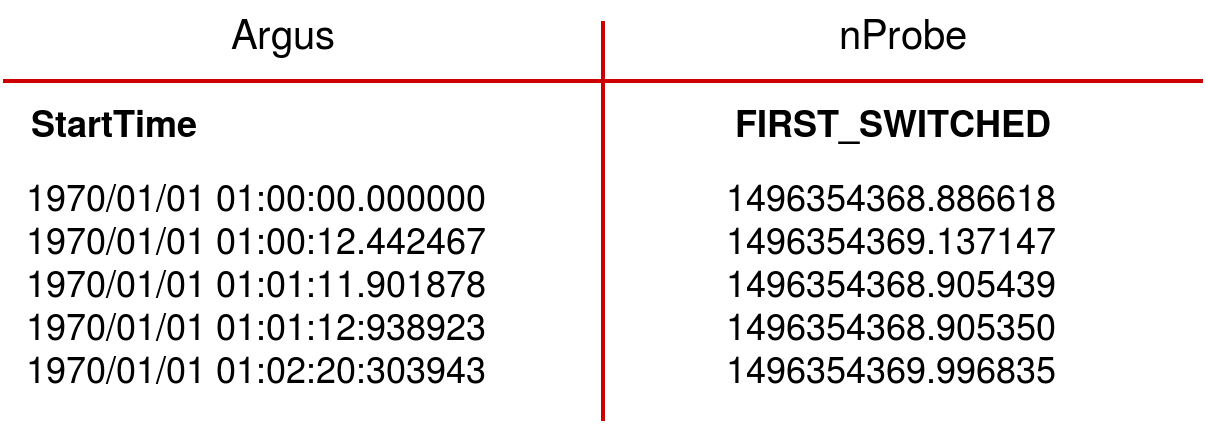
\includegraphics[scale=0.36]{starttime.png}
				\caption{Formattazione delle date}
				\label{fig:starttime}
\end{figure}
Argus salva la data seguita da uno spazio bianco, le ore i minuti e i secondi e i microsecondi. nProbe invece non salva la data ma soltanto i secondi nel formato $10^{10}$ con i microsecondi. Per effettuare una conversione precisa dei due campi la data nel formato YYYY/MM/DD è stata presa dalla struttura gerarchica delle cartelle guardando in modo ricorsivo la posizione del file all'interno del file system. Per i secondi si è convertito i 10 gigasecondi in secondi, mentre per i microsecondi non c'è stato bisogno di conversione.

Il secondo campo di Argus è \textit{Duration}. Non esistendo un campo di nProbe che indica la durata si è usata la differenza tra i campi \textit{LAST\_SWITCHED} e \textit{FIRST\_SWITCHED}. In figura ~\ref{fig:duration} viene mostrata l'operazione di differenza.
\begin{figure}[H]
				\centering
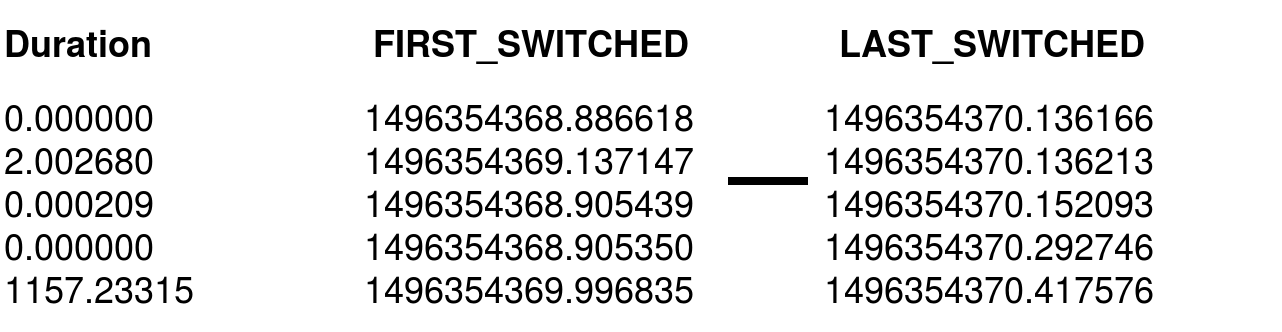
\includegraphics[scale=0.33]{duration.png}
				\caption{Durata}
				\label{fig:duration}
\end{figure}
Dopo aver fatto la differenza tra i due campi si converte il risultato in secondi e microsecondi per rispettare il formato di Argus.

Il terzo campo di Argus è \textit{Proto} che indica il protocollo usato dalla connessione. Argus salva in questo campo la keyword del protocollo mentre nProbe salva il numero decimale. La figura ~\ref{fig:protocol} mostra la differenza tra i due formati.
\begin{figure}[H]
				\centering
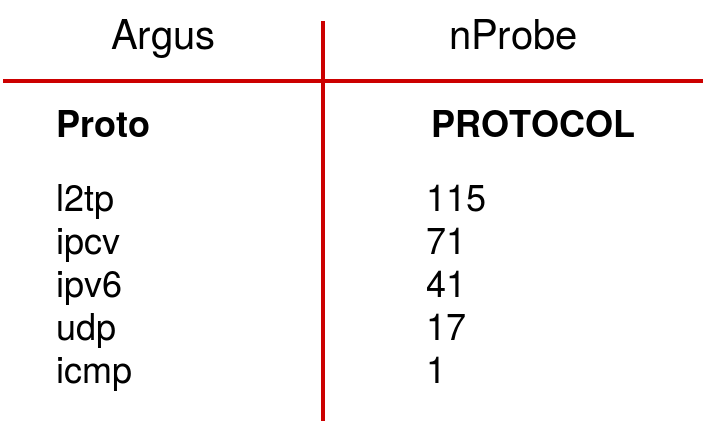
\includegraphics[scale=0.33]{protocol.png}
				\caption{Protocolli}
				\label{fig:protocol}
\end{figure}
Per effettuare la conversione tra numeri e keyword si è usato un \textit{dictionary}, un costrutto del linguaggio Python. Questa particolare struttura dati è un array associativo in cui una chiave viene associata ad un valore. Come chiave si è usato il numero decimale del protocollo e come valore la keyword. Il costo medio di accesso ad un valore con questa struttura dati è $\mathcal{O}(1)$. La figura ~\ref{lst:dictionary} rappresenta la sintassi di un dictionary in Python.
\lstinputlisting[language=Python, firstline=32, lastline=43, label={lst:dictionary}, caption={Esempio di dictionary}]{singlecore.py}

Il quarto campo di Argus è \textit{SrcAddr} che indica l'indirizzo IP sorgente. Questo campo è presente nei campi di nProbe, di conseguenza non è necessario effettuare una conversione. La figura ~\ref{fig:srcaddr} mette in evidenza i due formati.
\begin{figure}[H]
				\centering
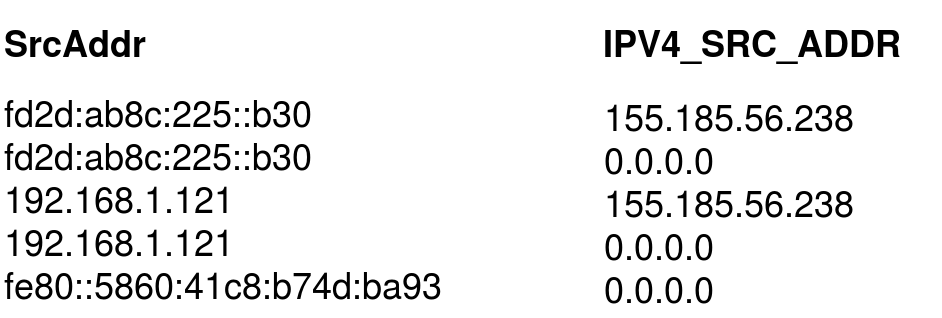
\includegraphics[scale=0.33]{srcaddr.png}
				\caption{Indirizzo IP sorgente}
				\label{fig:srcaddr}
\end{figure}

Il quinto campo di Argus è \textit{Sport} che indica la porta di origine della connessione. Il campo corrispettivo di nProbe è \textit{L4\_SRC\_PORT} e condividono entrambi lo stesso formato, non è pertanto necessario alcun tipo di conversione per questi due campi. La figura ~\ref{fig:sport} mostra i campi della porta sorgente nei due formati.
\begin{figure}[H]
				\centering
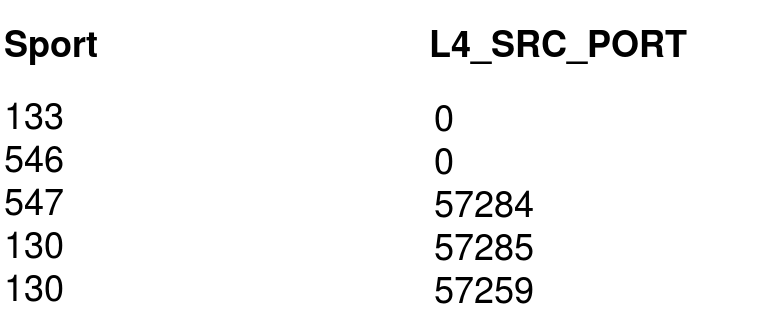
\includegraphics[scale=0.33]{sport.png}
				\caption{Porta sorgente}
				\label{fig:sport}
\end{figure}

Il sesto campo di Argus si chiama \textit{Dir} e rappresenta la direzione della connessione. Per la conversione si è utilizzato il campo di nProbe \textit{BIFLOW\_DIRECTION}. In nProbe si ha come valore del campo BIFLOW\_DIRECTION solo 1 e 2. Il numero 1 indica un flow monodirezionale che va dall'indirizzo sorgente al indirizzo destinazione, mentre il valore 2 indica un flow bidirezionale. In Argus si hanno più valori:
\begin{itemize}
				\item \textbf{-} la connessione è normale
				\item $\boldsymbol|$ la connessione è stata resettata
				\item \textbf{o} la connessione è scaduta
				\item \textbf{?} la direzione della connessione è sconosciuta
\end{itemize}

La figura ~\ref{fig:direction} mostra come è stata effettuata la conversione.
\begin{figure}[H]
				\centering
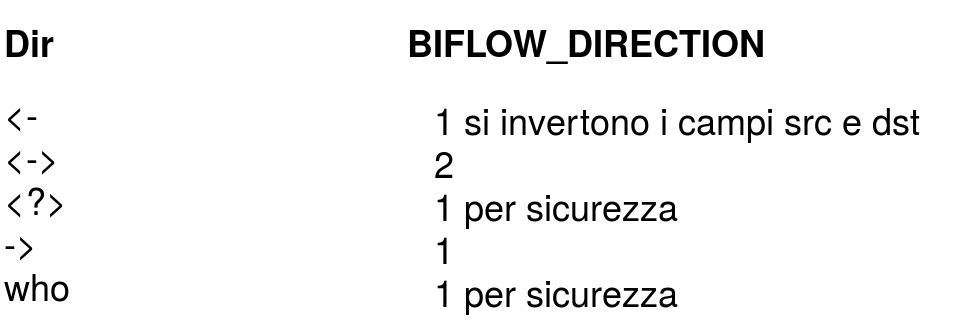
\includegraphics[scale=0.36]{direction.png}
				\caption{Direzione connessione}
				\label{fig:direction}
\end{figure}
Nel primo caso si può convertire con 1 ma bisogna invertire i campi src e dst perchè la connessione viene inizializzata a sinistra. Nel secondo caso si converte con due perchè il flow è bidirezionale. Nel terzo caso la direzione della connessione è sconosciuta, si è scelto di convertire con 1 per sicurezza e non lasciare il campo vuoto. Nel quarto caso il flow è monodirezionale e quindi si converte con 1. Nell'ultimo caso \textit{who} è una keyword che indica una comunicazione \textit{icmp} che non viene utilizzata da Stratosphere, si è scelto di convertire con 1 per sicurezza.

Il settimo campo di Argus è \textit{DstAddr} e rappresenta l'indirizzo IP di destinazione. Il campo corrispondente di nProbe si chiama \textit{IPV4\_DST\_ADDR}. La figura ~\ref{fig:dstaddr} mostra la formattazione dei dati. Come nel caso dell'indirizzo IP sorgente anche qui non è necessaria la conversione.
\begin{figure}[H]
				\centering
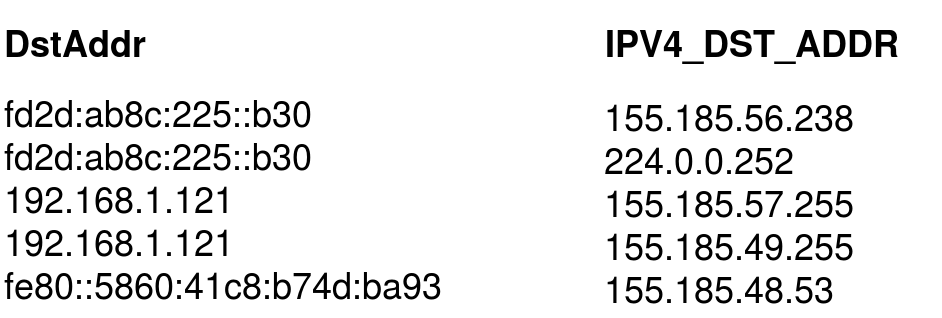
\includegraphics[scale=0.36]{dstaddr.png}
				\caption{Indirizzo IP destinazione}
				\label{fig:dstaddr}
\end{figure}

L'ottavo campo di Argus è \textit{Dport} e indica la porta di destinazione. Argus usa una formattazione decimale, stessa cosa il campo \textit{DST\_PORT} di nProbe. La figura ~\ref{fig:dport} mostra la formattazione dei campi. 
\begin{figure}[H]
				\centering
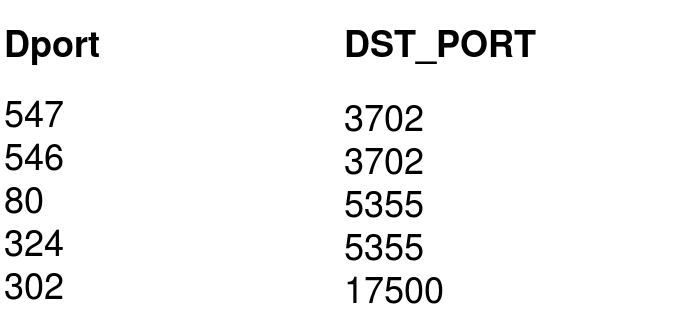
\includegraphics[scale=0.36]{dport.png}
				\caption{Porta di destinazione}
				\label{fig:dport}
\end{figure}

Il nono campo di Argus è \textit{State} e denota lo stato della connessione. Questo campo non è generabile a partire dai file di nProbe. Per effettuare questa conversione si è prima verificato l'impatto di questo campo nella generazione dei modelli di STF inserendo un valore non corretto. I modelli generati cambiando i valori di questo campo con valori non corretti restano invariati, pertanto il campo State non ne influenza la generazione. Per la conversione si è quindi inserito un valore costante "CON" per sicurezza. La figura ~\ref{fig:state} mostra esempi di valori del campo State di Argus.
\begin{figure}[H]
				\centering
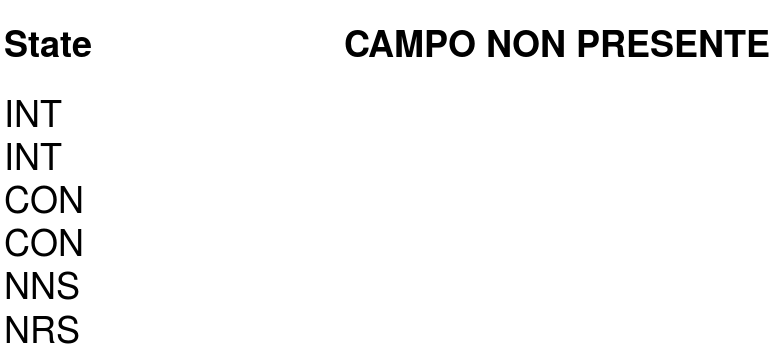
\includegraphics[scale=0.36]{state.png}
				\caption{Stato connessione}
				\label{fig:state}
\end{figure}

Il decimo e undicesimo campo di Argus sono \textit{sTos} \textit{dTos} e rappresentano il \textit{Type of Service} sorgente e destinazione di un pacchetto. Questi campi sono presenti in nProbe e condividono la stessa formattazione di Argus, non è pertanto necessaria una conversione. La figura ~\ref{fig:srctos} mostra esempi di valori di Type of Service.
\begin{figure}[H]
				\centering
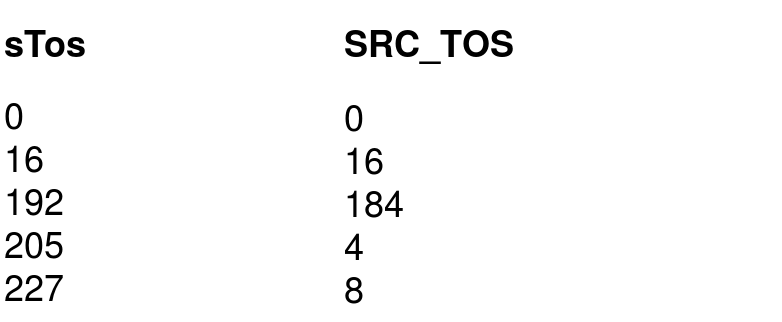
\includegraphics[scale=0.36]{srctos.png}
				\caption{Type of Service sorgente}
				\label{fig:srctos}
\end{figure}

Il dodicesimo campo di Argus è \textit{TotPkts} e rappresenta i pacchetti totali transitati nella connessione. Questo campo non compare in nProbe che ha però i campi \textit{IN\_PKTS} e \textit{OUT\_PKTS}. Per fare la conversione da nProbe ad Argus si sono sommati questi due valori per ottenere il totale dei pacchetti. La figura ~\ref{fig:totpkts} mostra l'operazione di somma e la formattazione dei dati.
\begin{figure}[H]
				\centering
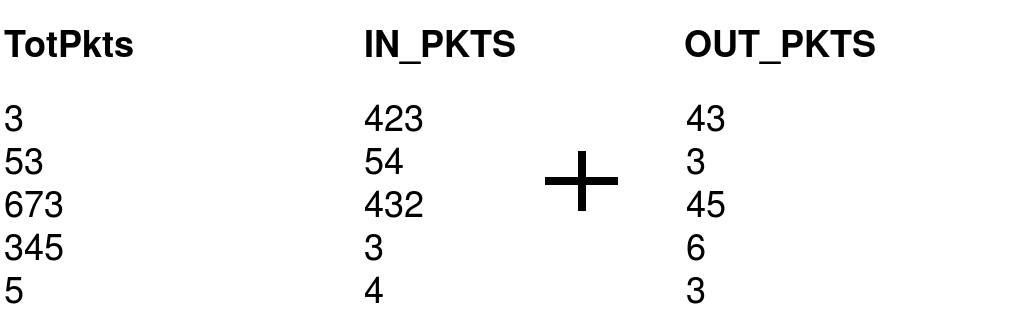
\includegraphics[scale=0.36]{totpkts.png}
				\caption{Pacchetti totali transitati nella connessione}
				\label{fig:totpkts}
\end{figure}

Il tredicesimo campo di Argus è \textit{TotBytes} e rappresenta i bytes totali transitati nella connessione. Come visto per il campo TotPkts, in nProbe questo campo non campare direttamente ma sono presenti \textit{IN\_BYTES} e \textit{OUT\_BYTES}. Per fare la conversione questi due campi vengono sommati per ottenere il totale. La figura ~\ref{fig:totbytes} mostra l'operazione di somma e la formattazione dei dati.
\begin{figure}[H]
				\centering
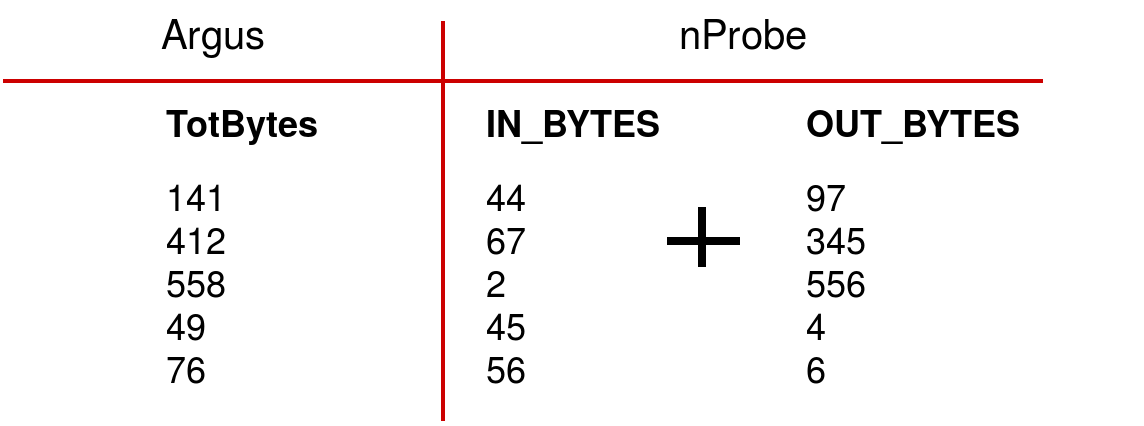
\includegraphics[scale=0.36]{totbytes.png}
				\caption{Bytes totali transitati nella connessione}
				\label{fig:totbytes}
\end{figure}

Il quattordicesimo campo di Argus è \textit{SrcBytes} che indica i bytes in entrata dal sorgente. Per fare questa conversione si è usato il campo di nProbe \textit{IN\_BYTES} in figura ~\ref{fig:totbytes}.

Il quindicesimo e ultimo campo di Argus è il campo label che serve per i metadata. Questo campo non è presente in nProbe e non è necessario per la generazione dei modelli, viene quindi lasciato vuoto.

La tabella ~\ref{table:tabellaConversione} riassume le scelte di conversione, mostra sulla colonna di sinistra i campi dell'header di Argus, mentre sulla destra i campi di nProbe. 
				\begin{table}[]
								\centering
								\begin{tabular}{|l|l|}
												\hline
												\multicolumn{1}{|c|}{\textbf{Argus}} & \multicolumn{1}{c|}{\textbf{nProbe}} \\ \hline
												StartTime                            & FIRST\_SWITCHED                      \\ \hline
												Duration                             & LAST\_SWITCHED - FIRST\_SWITCHED     \\ \hline
												Proto                                & PROTOCOL                             \\ \hline
												SrcAddr                              & IPv4\_SRC\_ADDR                      \\ \hline
												Sport                                & L4\_SRC\_PORT                        \\ \hline
												Dir                                  & BIFLOW\_DIRECTION                    \\ \hline
												DstAddr                              & IPv4\_DST\_ADDR                      \\ \hline
												Dport                                & DST\_PORT                            \\ \hline
												State                                & -                                    \\ \hline
												sTos                                 & SRC\_TOS                             \\ \hline
												dTos                                 & DST\_TOS                             \\ \hline
												TotPkts                              & IN\_PKTS + OUT\_PKTS                 \\ \hline
												TotBytes                             & IN\_BYTES + OUT\_BYTES               \\ \hline
												SrcBytes                             & IN\_BYTES                            \\ \hline
												Label                                & -                                    \\ \hline
								\end{tabular}
				\caption{Tabella di conversione}
								\label{table:tabellaConversione}
\end{table}


\section{Automatizzazione conversione}
La conversione è stata automatizzata con la scrittura di uno script in Python. Si è scelto di scrivere un programma usando questo linguaggio per la facilità di utilizzo nel lavorare con i file e per le performance.

Il problema richiede lo sviluppo di un programma che converte file in modalità batch.
La figura ~\ref{fig:lettura} rappresenta l'operazione da eseguire per la lettura dei file. I file, che sono organizzati in cartelle per data, sono presi in modo ricorsivo e inseriti in una coda. Al termine della lettura dei file si ha una coda con l'insieme dei path dei file da leggere.
\begin{figure}[H]
				\centering
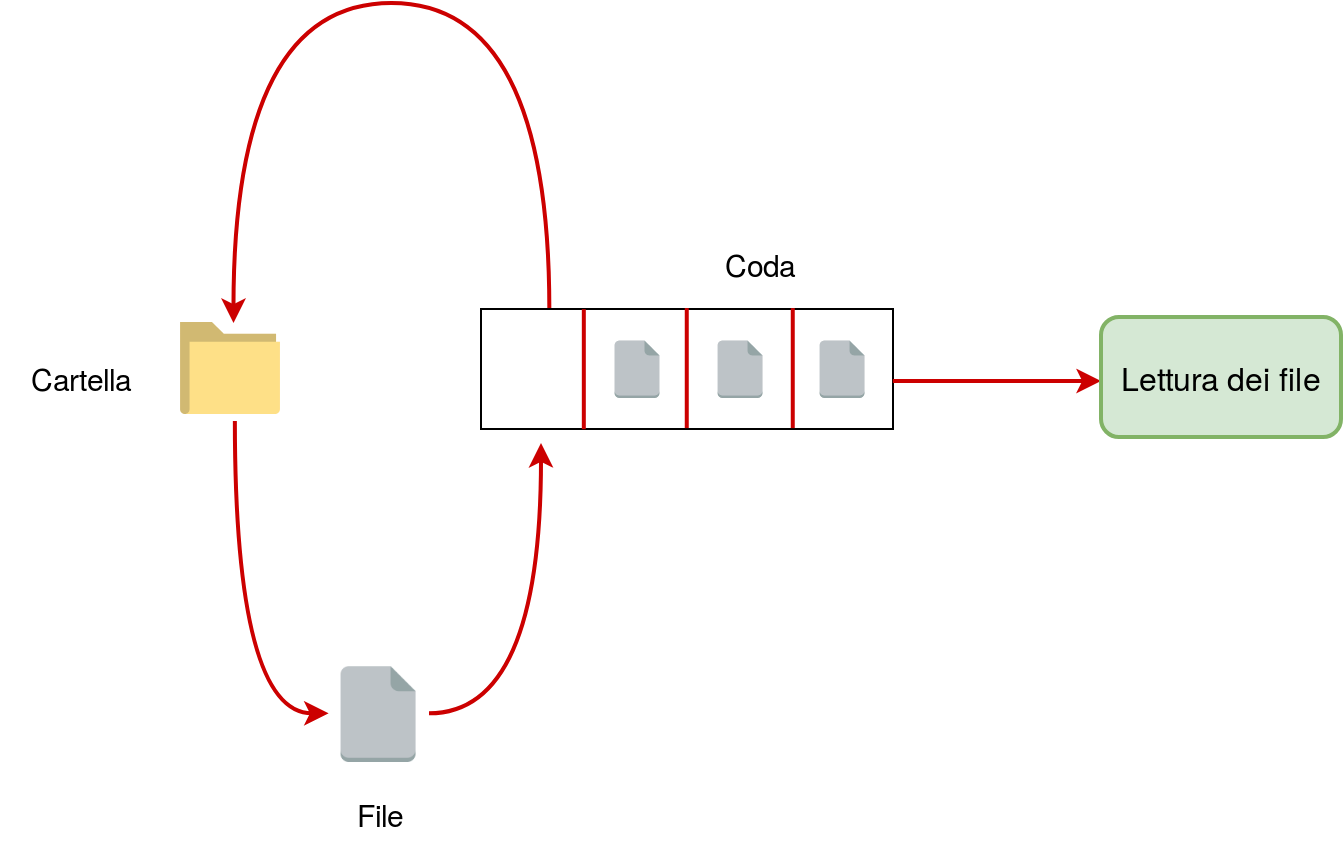
\includegraphics[scale=0.3]{lettura.png}
				\caption{Lettura dei file ricorsiva}
				\label{fig:lettura}
\end{figure}

Lo pseudocodice ~\ref{alg:ricorsione} descrive l'immagine ~\ref{fig:lettura}. Alla riga 1 si assegna ad una variabile il path della cartella in cui sono contenuti i file e nella seconda riga si crea un oggetto coda. Si creano poi due cicli for annidati che scorrono la struttura gerarchica della cartella e per ogni ogni file all'interno della cartella \textit{minuti} si mette in coda il file. Quando l'esecuzione dei due cicli for finisce rimane una coda con all'interno tutti i path dei file.
\begin{algorithm}
\caption{Inserimento file in una coda}
				\label{alg:ricorsione}
\begin{algorithmic}[1]
				\State $\textit{cartellaRoot} =  $\textit{pathCartella}
				\State $\textit{Coda} = $\textit{Queue()}
				\For{\texttt{mesi, giorni, minuti in \textit{cartellaRoot}}}
						\For{\texttt{file in minuti}}
						\State $\textit{Coda}.append() = $\textit{file}
						\EndFor
				\EndFor
\end{algorithmic}
\end{algorithm}

\begin{figure}[H]
				\centering
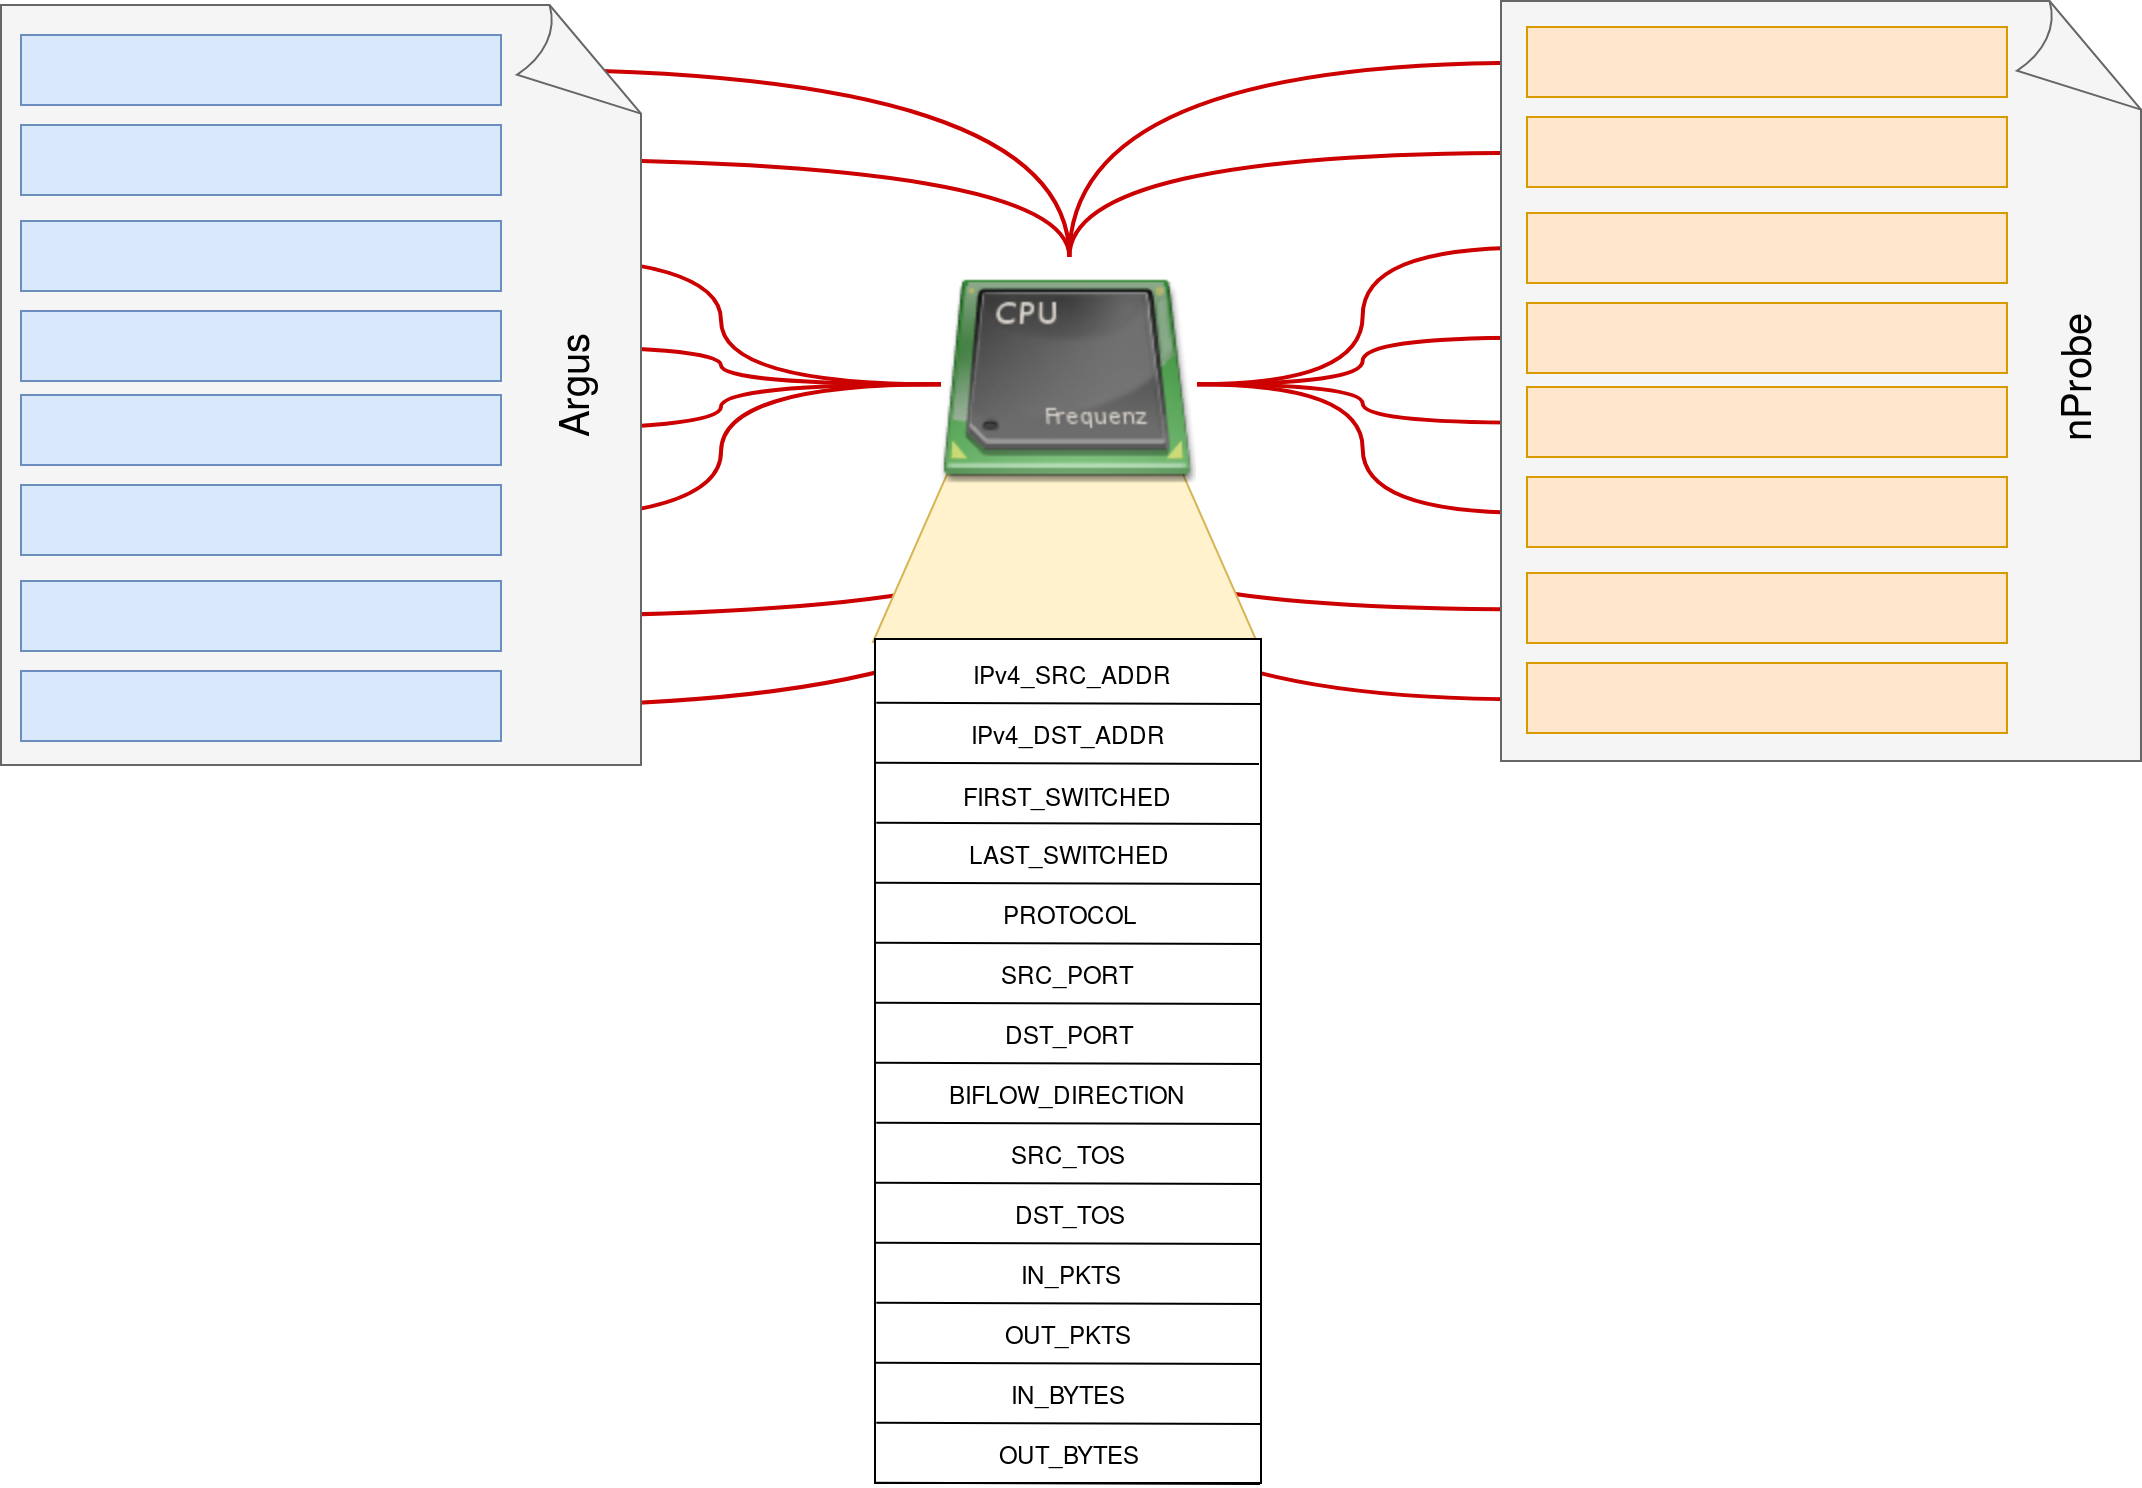
\includegraphics[scale=0.2]{letturarighe.png}
				\caption{Lettura dei file ricorsiva}
				\label{fig:letturarighe}
\end{figure}

Si è scelto di leggere il file una riga alla volta perchè le grandi dimensioni dei file non permettono un approccio diverso. Un approccio più veloce sarebbe stato quello di leggere i file per intero nella memoria principale ma non è un approccio possibile perchè possono presentarsi casi in cui la dimensione della RAM, soprattutto nei computer più datati, è più piccola rispetto a quella dei file.

L'algoritmo ~\ref{alg:singleCore} scritto in pseudocodice descrive una soluzione single core al problema

\begin{algorithm}
\caption{Single core version}
				\label{alg:singleCore}
\begin{algorithmic}[1]
\Procedure{Hydra}{}
\ForAll{\textit{file} in path}
\State read data from \textit{file}
\State convert data into new format
\State append data into new file
\EndFor

\EndProcedure
\end{algorithmic}
\end{algorithm}

\section{Rendere efficiente la conversione}

Nel programma descritto in precendenza viene generato un solo file di output in cui vengono convertiti tutti i file dati in input. Questa soluzione è comoda perchè da migliaia di file si ottiene un solo file con i dati convertiti, ma presenta il problema di creare un file con dimensioni enormi e di difficile gestione (il file può raggiungere dimensioni tali da rendere difficile anche solo aprirlo in lettura).


Il programma è inoltre inefficiente poichè è single core e ha come collo di bottiglia la scrittura su un unico file. 
La soluzione proposta seppure sia teoricamente corretta non può avere un'applicazione nel mondo reale. Bisogna cambiare quindi strategia per rendere la conversione più veloce sfruttando le macchine multi core e per avere in output file di dimensioni accettabili.

\subsection{Possibili soluzioni}
Si possono pensare diverse soluzioni che migliorerebbero in modo significativo il programma visto in precedenza:

\begin{itemize}
				\item Lavorare su chunk di file
				\item Meccanismi di lock
				\item Scrittura su file 1:1
\end{itemize}

\begin{verse}
\textbf{Lavorare su chunk di file}
Per velocizzare il programma e sfruttare i processori disponibili si potrebbe assegnare ad ogni processore un file da leggere e convertire. Quando il processore termina la conversione dei dati scrive sul file in output. In questo modo si dividrebbe il tempo di esecuzione sul numero di processori disponibili. 
Questa soluzione rende il più veloce possibile la conversione dei file ma i processori finiscono per scrivere sullo stesso file senza avere nessuna regola di precedenza, questo crea problemi perchè le scritture in output non sono ordinate e non è possibile creare modelli comportamentali affidabili. Le scritture su file devono essere ordinate e sequenziali, inoltre questa soluzione ha il problema di scrivere sempre su unico file e come detto in precedenza questo tipo di soluzione non è possibile.
\end{verse}

\begin{verse}
\textbf{Meccanismi di lock}
Un modo per risolvere i problemi precedenti è quello di utilizzare il concetto di semaforo. 
In informatica un semaforo è un tipo di dato astratto gestito da un sistema operativo multitasking per sincronizzare l'accesso a risorse condivise tra processi. È composto da una variabile intera e da una coda di processi. Quando un processo apre il file per scriverci viene impostato un semaforo che segnala che la risorsa è occupata, se un altro processore prova ad aprire lo stesso file per scriverci gli sarà negato l'accesso dal semaforo fino a quando l'altro processo non rilascerà la risorsa.
In questo modo si risolve il problema delle scritture ordinate, ma c'è da tener conto che i semafori riducono la velocità di esecuzione dell'algoritmo poichè mentre un processore occupa la risorsa tutti gli altri processori devono mettersi in coda per aspettarne il rilascio. Nonostante questa soluzione rallenti l'esecuzione del programma rispetto alla soluzione precedente è comunque molto più veloce della versione single core perchè, sebbene la scrittura su file sia rallentata dai semafori, si guadagna molto tempo nella lettura e conversione dei dati dove non ne è necessario l'utilizzo, e che quindi viene effettuata alla massima velocità possibile. Questa soluzione risolve anche il problema dell'ordinamento delle scritture.
Rimane il problema della scrittura su un unico file che però può essere risolto facilmente decidendo di scrivere su un nuovo file quando raggiunge una dimensione specificata.
Se si implementa la divisione del file di output questa soluzione può considerarsi efficiente anche se rimane il collo di bottiglia introdotto dai semafori che costringe i processi ad aspettare in coda quando una risorsa è impegnata.
\end{verse}

\begin{verse}
\textbf{Scrittura su file 1:1}
In questa soluzione ogni processore apre un file, lo legge, lo converte e scrive su un proprio file.
Questa soluzione è decisamente la più semplice tra quelle proposte ed è anche la più efficiente poichè i processori non entrano mai in conflitto tra di loro cosicchè da effettuare letture, conversioni e scritture alla massima velocità possibile dalla macchina.
Un problema che può creare questa soluzione è la produzione di una grande quantità di file in output. Si pensi che una sola settimana di traffico di rete, sono circa 10 mila file.
\end{verse}

\subsection{Scelta effettuata}

Si è scelto di procedere con l'ultima soluzione presentata perchè data la grande quantità di informazioni da convertire si preferisce l'approccio più veloce a discapito dell'ordinamento finale.

Il programma, dato in input la root directory dei file, cerca ricorsivamente tutti i file e li inserisce in una coda, chiama poi una funzione a cui assegna 4 processori. La funzione ha un ciclo while che si ripete fino a quando la coda popolata da tutti i file non è vuota. Ogni processore che entra in questa funzione toglie un file dalla coda e lo elabora.

Il programma ~\ref{alg:multiCore} descrive una soluzione multi core
\begin{algorithm}
\caption{Multi core version}
				\label{alg:multiCore}
\begin{algorithmic}[1]
\Procedure{Hydra}{}
\ForAll{\textit{file} in path}
\State $\textit{Queue[]} \gets \textit{file}$
\State read data from $\textit{file}$
\State spawn 4 process
\While{\textit{Queue[]} $\textbf{not empty}$}
\State $\textit{filename} \gets $\textit{Queue.get()}
\State convert data into new format
\State append data into new file
\EndWhile
\EndFor
\EndProcedure
\end{algorithmic}
\end{algorithm}
\end{document}

La figura ~\ref{fig:multiCore} descrive lo pseudocodice del programma parallelo. Ogni file da convertire è inserito in una coda a cui accedono i processori, ogni processore lavora individualmente sul proprio file da cui legge e converte i dati. La scrittura su file rimane indipendente perchè ogni processore lavora sul proprio file.

\begin{figure}[H]
				\centering
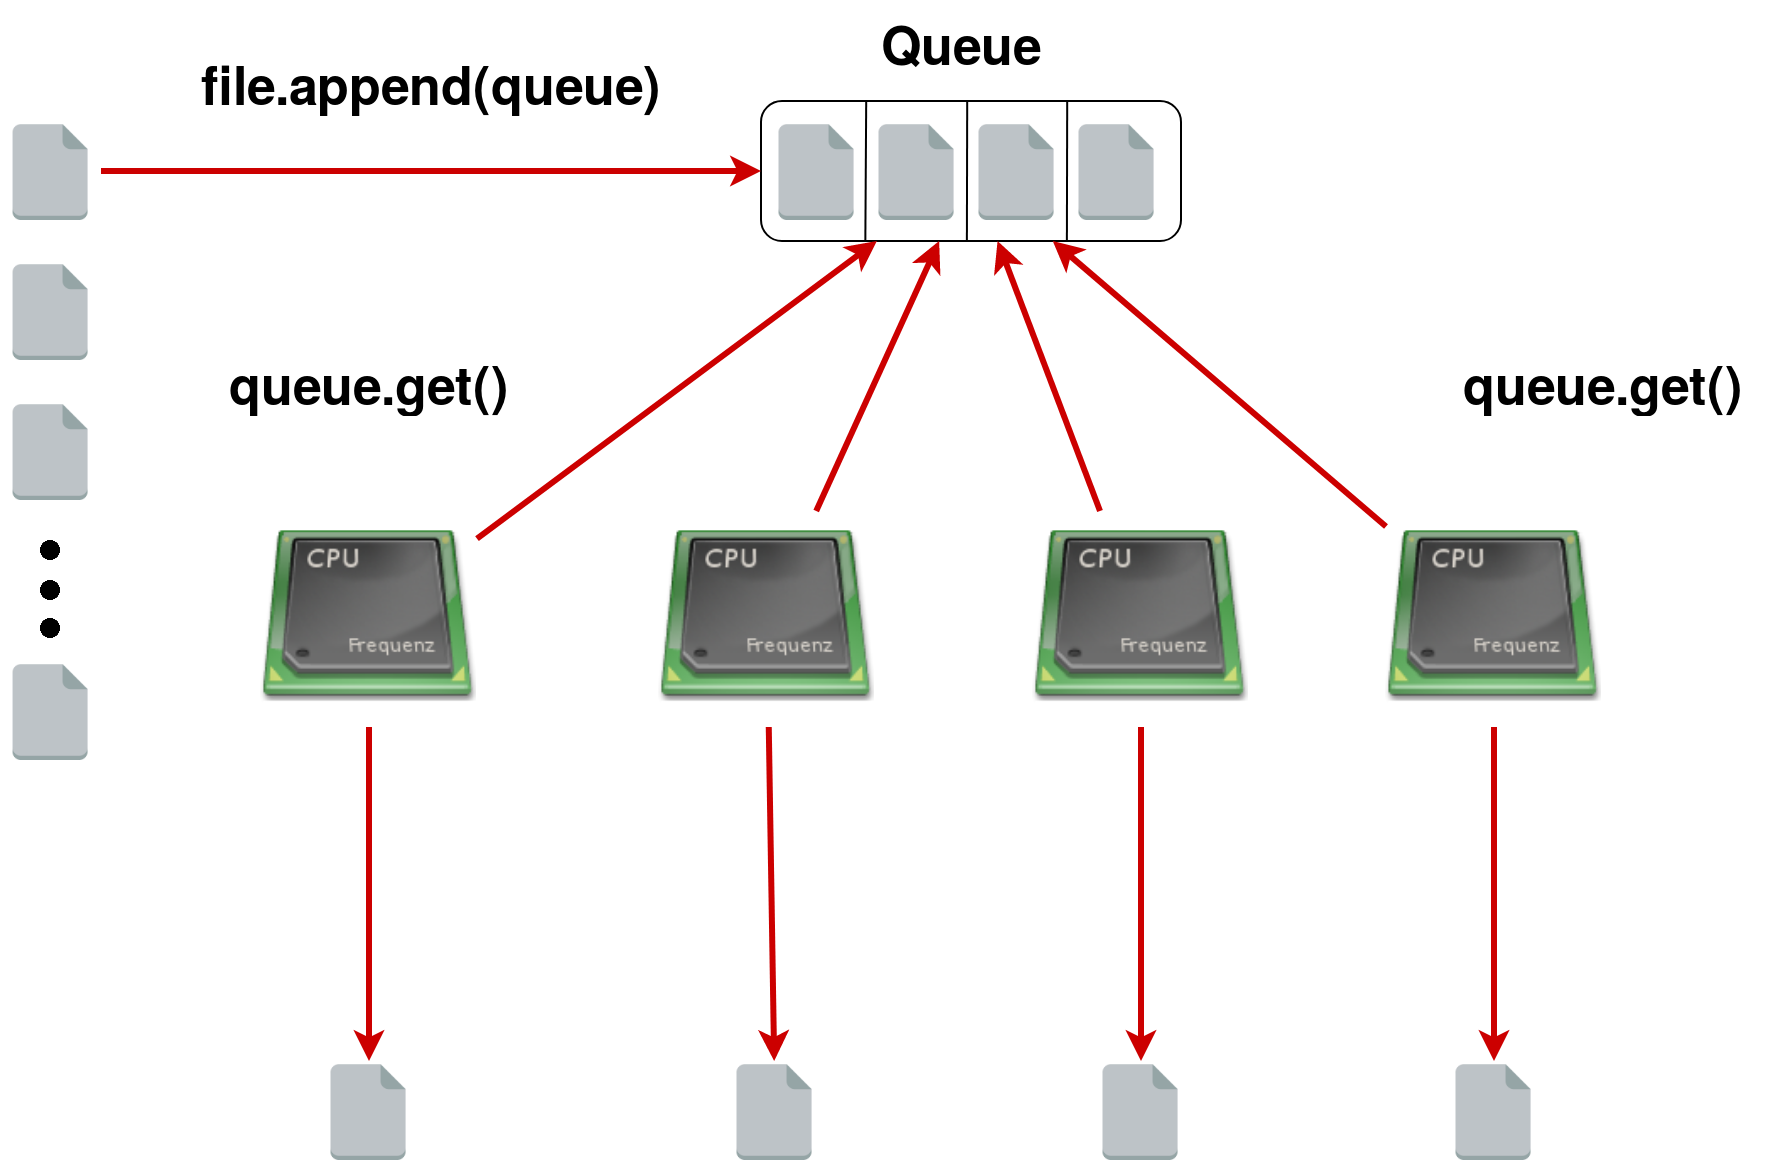
\includegraphics[scale=0.22]{hydra.png}
				\caption{Multi core version}
				\label{fig:multiCore}
\end{figure}


